\chapter{Environment\label{chap:env}}

This chapter describes the software environment (section \ref{sec:simulation}) 
the different models were developed and tested in. Furthermore section 
\ref{sec:usedTec} describes the important technologies that were used.

\section{Simulation\label{sec:simulation}}

The model is supposed to learn object manipulation through interaction. Instead of on a real robot the model has been developed and tested in a simplified simulation. For this work gazebo \cite{gazebo} V.2.2.3 was used with the physics engine Open Dynamics Engine (ODE) \cite{ode}. This simulation and version were chosen because this thesis was initially planned as a part of a bigger project in the Citec of Bielefeld University where this software was used as well. 

\subsection{World and robot actions}%TODO Check if remained the same

The model was developed with a toy-world consisting of only a sphere, which is 
regarded as actuator, and a rectangular block as can be seen in figure 
\ref{fig:gazeboWorld}.
Since the focus of this work is to learn simple object interactions, the 
possible actions of the robot were limited to moving the actuator freely in two 
dimensions.

\begin{figure} %TODO Check if remained the same
	%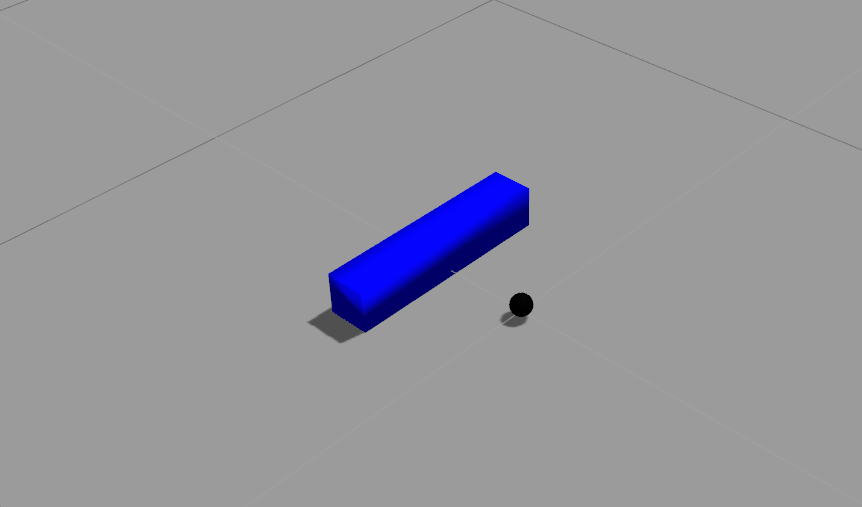
\includegraphics[width=5cm]{images/gazeboWorld.png} %TODO make image
	\caption{Overview of the used world and objects. The sphere represents the 
	robot's actuator and the rectangular block represents the primary object.}
	\label{fig:gazeboWOrld}
\end{figure}


\subsection{Communication}
In order to communicate with the simulation, a plug-in was written, that publishes the properties of all objects using google protobuf \cite{protobuf}. These messages are received and unpacked by a custom python interface that handles the communication with the simulation from the model's side. The plug-in also interprets the commands coming from the interface. A list of all implemented commands can be found in table \ref{tab:commands}

\begin{table}
	\centering
\begin{tabular}{|c|c|}
	\hline \textbf{Command} & \textbf{Meaning} \\ 
	\hline Move Command & Sets the velocity for the actuator \\ 
	\hline Pause & Pauses the simulation \\
	\hline Unpause & Continues the simulation \\
	\hline Reset & Resets the world to starting configuration \\
	\hline Set Pose & Places a specified object at a certain position \\
	\hline
\end{tabular} 
\caption{Overview of all the commands implemented in the model.}
\label{tab:commands}
\end{table}



\section{Technologies\label{sec:usedTec}}

This section briefly describes the technologies that were used or adapted to 
build the model.

\subsection{Case based Reasoning\label{sec:CBR}}
%TODO make properly!
Case based reasoning (CBR) is a delayed...
In CBR a case, in this case an episode, consists of an initial state, an 
optional action or event, and the resulting state after the action or event has 
taken place. In CBR these cases are simply stored. Whenever a new situation is 
to be handled, the case whose initial state and action are most similar to the 
current situation and available actions is retrieved and the resulting state is 
used to make a prediction about the effect of each action. Inversely, by 
searching for the resulting states, one can also decide what kind of actions 
should be taken in order to achieve a certain desired state. 


\subsection{Instantaneous Topological Map \label{sec:ITM}}
Talk about :
\begin{itemize}
	\item Similarity/difference to GNG
	\item Extension to provide output
	\item How is it trained
	\item How does it make predictions
	\item How does it return an action/preconditions
\end{itemize}

\subsection{Decision Tree}

\subsection{Learning Vector Quantization}